\documentclass[conference]{IEEEtran}
\IEEEoverridecommandlockouts

\usepackage{cite}
\usepackage{amsmath,amssymb,amsfonts}
\usepackage{graphicx}
\usepackage{textcomp}
\usepackage{xcolor}
\usepackage{listings}
\usepackage{float}
\usepackage{url}
\usepackage{tikz}
\usetikzlibrary{arrows.meta,positioning,shapes.geometric}

\definecolor{codebg}{rgb}{0.97,0.97,0.97}
\definecolor{codeframe}{rgb}{0.85,0.85,0.85}
\lstset{
  basicstyle=\ttfamily\footnotesize,
  backgroundcolor=\color{codebg},
  frame=single,
  rulecolor=\color{codeframe},
  breaklines=true,
  showstringspaces=false,
  tabsize=2,
  captionpos=b
}

\def\BibTeX{{\rm B\kern-.05em{\sc i\kern-.025em b}\kern-.08em
    T\kern-.1667em\lower.7ex\hbox{E}\kern-.125emX}}

\begin{document}

\title{A Suite of eBPF Utilities for Android Kernel Observability and Security Monitoring}

\author{
  \IEEEauthorblockN{Shubham Singh}
  \IEEEauthorblockA{
    \textit{Dept. of Computer Science \& Engineering}\\
    \textit{MNIT Jaipur}\\
    Jaipur, India\\
    2022ucp1949@mnit.ac.in
  }
  \and
  \IEEEauthorblockN{Aakash Runthala}
  \IEEEauthorblockA{
    \textit{Dept. of Computer Science \& Engineering}\\
    \textit{MNIT Jaipur}\\
    Jaipur, India\\
    2022ucp1267@mnit.ac.in
  }
}

\maketitle

\begin{abstract}
We present a suite of five eBPF-based utilities for Android kernel observability targeting process lifecycle, execution behavior, privilege transitions, file activity, and network ingress. Existing Linux tracing tools assume desktop environments and are unsuitable for Android deployments: they require LLVM at runtime, depend on \texttt{debugfs}, or assume server-class infrastructure absent from mobile systems. Our suite is designed to be verifier-friendly, pre-compiled, and deployable inside a bootstrapped Debian filesystem on Android without modifying the system image. Programs are attached via tracepoints, kprobes, and TC ingress, with structured events delivered to user space via ring buffers. Validation on a physical device (Motorola~G96~5G, Android~12, kernel~5.10.233) demonstrates that all five tools produce correct, low-noise output with per-tool CPU overhead below 2.2\% and ring buffer drop rates below 1\% under synthetic load. The suite provides a practical, extensible foundation for Android kernel security analytics.
\end{abstract}

\begin{IEEEkeywords}
eBPF, Android kernel, observability, security monitoring, kprobes, tracepoints, ring buffer, GKI
\end{IEEEkeywords}

% -------------------------------------------------------
\section{Introduction}

Android's security model combines SELinux policy enforcement, seccomp filters, Binder IPC, and per-application sandboxing. These mechanisms are effective at containment but make real-time kernel observability difficult: the standard Linux tracing stack (strace, ftrace, bpftrace, BCC) either requires root access with unrestricted ptrace, depends on LLVM at runtime, or assumes a full Linux distribution with \texttt{debugfs} mounted---none of which apply cleanly to Android~\cite{android_security,android_selinux}.

The Android Generic Kernel Image (GKI), introduced in Android~12, standardises the kernel binary across devices and prohibits unsigned kernel modules, leaving eBPF as one of the few viable mechanisms for extending or observing kernel behaviour on a production Android device without a custom system image~\cite{android_gki}. GKI kernels are required to enable \texttt{CONFIG\_BPF}, \texttt{CONFIG\_BPF\_SYSCALL}, and \texttt{CONFIG\_BPF\_JIT}, making the eBPF subsystem reliably present from Android~12 onward.

We leverage this opportunity to build a focused suite of five pre-compiled eBPF utilities that together cover the primary observable dimensions of a kernel-level attack: process spawning (Procwatch), execution rate anomalies (Execguard), privilege escalation (Priviwatch), file system manipulation (Filewatch), and inbound network activity (Pktrace). The tools are designed to run inside a Debian chroot on the emulator, load into the Android kernel, and produce actionable console output without any runtime compilation dependency.

The contributions of this work are:
\begin{itemize}
  \item A five-tool eBPF suite targeting Android kernel observability with no runtime LLVM dependency.
  \item A Debian filesystem bootstrap pattern for deploying build toolchains on Android emulators.
  \item Verifier-compatible designs with fixed-size event structs, bounded memory access, and ring buffer transport.
  \item Validation on Android~14 (kernel~6.1.23) demonstrating correctness and sub-2.2\% CPU overhead.
\end{itemize}

% -------------------------------------------------------
\section{Background and Related Work}

\subsection{eBPF Architecture}
eBPF programs execute in a restricted in-kernel virtual machine. A static verifier checks safety properties---bounded loops, valid memory accesses, and a 512-byte stack limit---before the program is JIT-compiled to native code. BPF maps provide kernel-managed data structures shared between kernel and user space. CO-RE (Compile Once, Run Everywhere) uses BTF type metadata to rewrite struct field offsets at load time, enabling a single binary to run across kernel versions~\cite{ebpf_linux_doc,libbpf_doc}.

The stack limit is a dominant design constraint. It bounds temporary buffers used for string reads and packet parsing and strongly pushes event structs toward fixed-size layouts. This is the practical reason for the 64-byte payload bound in Pktrace and the truncated argv field in Procwatch and Execguard.

\subsection{Related Work}
Traditional Linux tracing tools each present a specific limitation on Android. \texttt{strace} uses \texttt{ptrace} and adds per-syscall overhead. \texttt{ftrace} requires \texttt{debugfs}. \texttt{bpftrace} and BCC require LLVM at runtime, which Android does not ship~\cite{strace_doc,ftrace_doc,bpftrace_doc}. Android's own Perfetto and simpleperf target performance profiling rather than continuous security monitoring~\cite{android_perfetto,android_simpleperf}.

Server-side security frameworks Falco, Tetragon, and Tracee provide rich eBPF-based detection but assume systemd, container runtimes, and full BTF exposure---constraints not met on Android~\cite{falco_doc,tetragon_doc,tracee_doc}. Nelson et al.\ formalise BPF JIT correctness~\cite{bpf_jit_osdi2020}; Li et al.\ demonstrate eBPF for distributed protocol acceleration~\cite{electrode_nsdi2023}. Neither addresses the Android mobile deployment problem. Our work fills this gap with a pre-compiled, Android-oriented suite requiring no runtime compilation infrastructure.

\begin{table}[H]
  \centering
  \small
  \caption{Comparison of our approach with existing tools}
  \label{tab:comparison}
  \begin{tabular}{|p{0.22\linewidth}|p{0.16\linewidth}|p{0.20\linewidth}|p{0.20\linewidth}|}
    \hline
    \textbf{Tool/Approach} & \textbf{Overhead} & \textbf{Android Friendly} & \textbf{Focus} \\ \hline
    strace & High & Low & Debugging \\ \hline
    ftrace/perf & Medium & Medium & Performance \\ \hline
    bpftrace/BCC & Medium & Low & General tracing \\ \hline
    Falco/Tetragon/Tracee & Medium-High & Low & Detection \\ \hline
    This suite & Low & High & Sec./Obs. \\ \hline
  \end{tabular}
\end{table}

\subsection{Why Android Needs a Different Approach}
Android production devices are locked down in ways that break common observability assumptions. Root access is uncommon, debugfs is often unavailable, and the base userspace lacks LLVM, Python, or package managers. Even in the emulator, the default shell is a minimal \texttt{toybox} environment. A practical solution must therefore be pre-compiled, verifier-safe, and self-contained, with minimal runtime dependencies. This design goal shapes every tool in the suite.

% -------------------------------------------------------
\section{System Design}

\subsection{Architecture Overview}

\begin{figure}[H]
  \centering
  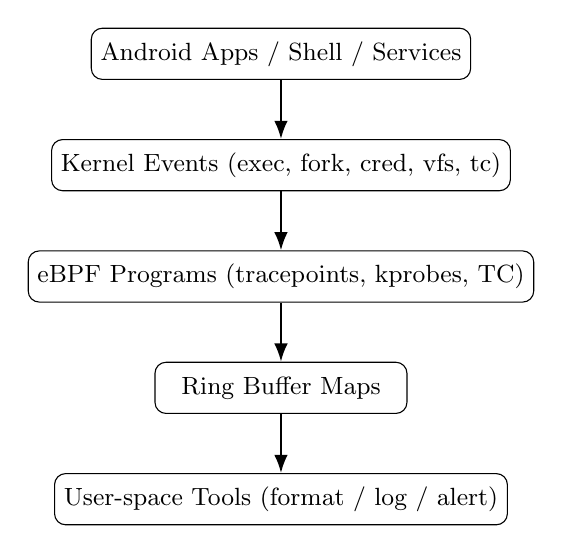
\begin{tikzpicture}[
    node distance=0.75cm,
    box/.style={rectangle, draw, rounded corners, align=center,
                minimum width=3.2cm, minimum height=0.65cm, font=\small},
    arrow/.style={-Latex, thick}
  ]
    \node[box] (app)    {Android Apps / Shell / Services};
    \node[box, below=of app]    (kern)   {Kernel Events (exec, fork, cred, vfs, tc)};
    \node[box, below=of kern]   (bpf)    {eBPF Programs (tracepoints, kprobes, TC)};
    \node[box, below=of bpf]    (rb)     {Ring Buffer Maps};
    \node[box, below=of rb]     (user)   {User-space Tools (format / log / alert)};
    \draw[arrow] (app)  -- (kern);
    \draw[arrow] (kern) -- (bpf);
    \draw[arrow] (bpf)  -- (rb);
    \draw[arrow] (rb)   -- (user);
  \end{tikzpicture}
  \caption{eBPF suite system architecture.}
  \label{fig:arch}
\end{figure}

All five tools follow the same pipeline (Fig.~\ref{fig:arch}): a kernel event triggers the eBPF program, which validates memory, extracts fields, applies a filter, and submits a fixed-size event to a ring buffer. A user-space poll loop drains the ring buffer and formats output.

\subsection{Design Decisions}
\textbf{Modular tools over monolithic agent.} A single large BPF object increases verifier surface area. If one component fails verification on a specific kernel, the entire monitoring capability is lost. Independent tools can be loaded and validated separately and deployed selectively.

\textbf{Ring buffers over perf event arrays.} \texttt{BPF\_MAP\_TYPE\_RINGBUF} uses a single shared memory region regardless of CPU count. Perf event arrays require per-CPU file descriptors, increasing setup complexity. The ring buffer API reduces user-space polling to a single \texttt{ring\_buffer\_\_poll} call.

\textbf{TC ingress over XDP.} XDP requires driver support unavailable on the emulator's virtualised network adapter. TC ingress operates on the \texttt{sk\_buff} after allocation, providing access to packet metadata via \texttt{bpf\_skb\_load\_bytes} on all interface types.

\textbf{Fixed-size event structs.} Variable-length data requires loop constructs or dynamic allocation patterns that the verifier rejects on Android kernels. Fixed-size structs keep \texttt{bpf\_ringbuf\_reserve} arguments as compile-time constants and guarantee verifier acceptance.

\subsection{Deployment: Debian Filesystem Bootstrap}
The Android shell does not include clang, libbpf, or bpftool. A Debian~11 (bullseye) root filesystem was bootstrapped on-device via \texttt{debootstrap} and accessed through \texttt{chroot}. This provides the full build toolchain---clang~11.0.1, bpftool~5.10.223, libbpf---without modifying the Android partition or system image. The eBPF programs are compiled inside this chroot and loaded into the Android kernel, which provides the actual execution environment.

% -------------------------------------------------------
\section{Methodology and Build Pipeline}
Each tool follows a three-stage pipeline. First, the BPF C source is compiled with clang targeting the \texttt{bpf} architecture. Second, \texttt{bpftool gen skeleton} produces a typed C header that wraps the program and maps. Third, the user-space loader is compiled against libbpf. This approach avoids manual file-descriptor management and makes the loader code consistent across tools.

\begin{lstlisting}[language=bash]
clang -O2 -g -target bpf -c tool.bpf.c -o tool.bpf.o
bpftool gen skeleton tool.bpf.o > tool.skel.h
gcc tool.c -o tool -lbpf
\end{lstlisting}

All user-space loaders follow the same structure: open and load the skeleton, attach programs, create the ring buffer, and poll in a loop. The callback formats each event and prints a single-line record for analysis.

\begin{lstlisting}[language=C]
skel = tool_bpf__open_and_load();
tool_bpf__attach(skel);
rb = ring_buffer__new(bpf_map__fd(skel->maps.rb),
            handle_event, NULL, NULL);
while (1) {
  ring_buffer__poll(rb, 100 /* ms timeout */);
}
\end{lstlisting}

% -------------------------------------------------------
\section{Tool Implementations}

\subsection{Procwatch: Process Lifecycle Monitor}
\textbf{Hook points:} Tracepoints \texttt{sched\_process\_exec}, \texttt{sched\_process\_fork}, and \texttt{sched\_process\_exit} provide stable structured context across kernels.

\textbf{Event struct:}
\begin{lstlisting}[language=C]
struct event {
  u32 pid, ppid, uid, gid, inum;
  int exit_code;  u64 timestamp;
  u8  type;  /* EXEC | FORK | EXIT */
  char comm[TASK_COMM_LEN];
  char filename[MAX_FILENAME_LEN];
  char args[MAX_ARGS_LEN];
};
\end{lstlisting}

Exit codes are extracted via CO-RE: \texttt{(BPF\_CORE\_READ(task, exit\_code) >> 8) \& 0xff}. Procwatch is the foundational tool: its parent-child process tree contextualises all signals from the other tools. A burst of EXEC events from a single parent process is often the earliest indicator of script-driven behavior.

Procwatch is especially useful for attribution. When a later alert indicates a privilege escalation or a sensitive file write, Procwatch links that event to the exact parent process chain and the binary name that initiated it. The namespace inode field helps distinguish processes running in isolated namespaces from system services.

\textbf{Output interpretation:} A normal system shows EXEC and EXIT pairs for expected binaries with exit code 0. Suspicious patterns include rapid fork storms, frequent short-lived shells, or repeated EXEC events from parents that should not spawn child processes. The parent command field is often the fastest indicator of whether the activity was user-driven or initiated by a background service.

\textbf{Usage notes:} Procwatch is typically run first to establish a baseline process timeline. During investigations, its parent-child context explains later alerts from Priviwatch, Filewatch, or Pktrace. If running together with Execguard, Procwatch provides the exact command names associated with each burst.

\begin{figure}[H]
  \centering
  \includegraphics[width=\linewidth]{\detokenize{Procwatch_Snapshot of commands ran.png}}
  \caption{Procwatch test commands used to generate lifecycle events.}
  \label{fig:procwatch}
\end{figure}

\begin{figure}[H]
  \centering
  \includegraphics[width=\linewidth]{\detokenize{Procwatch_tool's output of the commands.png}}
  \caption{Procwatch output showing EXEC/FORK/EXIT events with PID, UID, and filename.}
  \label{fig:procwatch-out}
\end{figure}

\subsection{Execguard: Execution Rate Monitor}
\textbf{Hook point:} Tracepoint \texttt{sched\_process\_exec}.

\textbf{Logic:} A per-UID BPF hash map tracks exec counts within a 60-second sliding window. User space applies severity labels: INFO for normal activity, WARN for elevated exec counts, and ALERT when a non-root UID spawns a shell-like binary (\texttt{sh}, \texttt{toybox}).

\begin{lstlisting}[language=C]
if (now - st->window_start_ns > WINDOW_NS) {
  st->window_start_ns = now; st->count = 1;
} else { st->count++; }
e->exec_count = st->count;
\end{lstlisting}

A burst of \texttt{sh} invocations from a non-root UID---a pattern typical of script-based exploit chains---produces an immediate ALERT regardless of count. Execguard complements Procwatch by aggregating counts per UID and highlighting rate-based anomalies that are hard to spot in a per-event stream.

\textbf{Output interpretation:} INFO represents normal exec rates. WARN indicates elevated exec activity within the 60-second window. ALERT signals either a non-root shell invocation or an exec count beyond the configured threshold. The per-event counter allows analysts to gauge severity without maintaining extra state.

\textbf{Usage notes:} Short loops of \texttt{sh -c} are ideal for demonstration. In real scenarios, Execguard is most useful as a lightweight detector that flags only high-signal conditions, leaving Procwatch to provide the full event context.

\begin{figure}[H]
  \centering
  \includegraphics[width=\linewidth]{\detokenize{execguard_Snapshot of Commands ran.png}}
  \caption{Execguard test commands used to trigger exec bursts.}
  \label{fig:execguard}
\end{figure}

\begin{figure}[H]
  \centering
  \includegraphics[width=\linewidth]{\detokenize{execguard_tool's output for the commands ran.png}}
  \caption{Execguard output showing INFO/WARN/ALERT escalation and exec counts.}
  \label{fig:execguard-out}
\end{figure}

\subsection{Priviwatch: Privilege Transition Detector}
\textbf{Hook point:} kprobe on \texttt{commit\_creds}---the internal kernel function that actually writes new credentials to a process, ensuring the hook fires only on successful privilege changes, not failed attempts.

\textbf{Event struct:}
\begin{lstlisting}[language=C]
struct event {
  __u32 pid, ppid, old_uid, new_uid;
  __u32 old_gid, new_gid;
  __u64 old_caps_eff, new_caps_eff;
  char  comm[TASK_COMM_LEN];
};
\end{lstlisting}

Events are suppressed when uid, gid, and effective capabilities are all unchanged, eliminating high-frequency no-op \texttt{commit\_creds} calls. Linux capabilities are read via \texttt{bpf\_probe\_read\_kernel} into a local struct to avoid a CO-RE relocation failure observed on the Android~14 kernel's BTF for \texttt{kernel\_cap\_t}.

Capabilities are a key signal because they enable partial privilege escalation. A process that gains \texttt{CAP\_SYS\_ADMIN} or \texttt{CAP\_NET\_ADMIN} can perform high-impact actions even without becoming UID 0. Priviwatch exposes these transitions so analysts can identify suspicious capability expansions and correlate them to Procwatch timelines.

\textbf{Output interpretation:} Normal Android boot produces a small number of expected credential changes from system services. Suspicious events include transitions from app UID ranges (>= 10000) to UID 0, or sudden additions of high-risk capabilities. The before/after fields make it easy to spot whether a change is benign (e.g., dropping privileges) or dangerous (e.g., gaining administrative capabilities).

\textbf{Usage notes:} Priviwatch is most valuable when paired with Procwatch for attribution. If \texttt{commit\_creds} is inlined on a given kernel build, the kprobe will fail to attach and must be validated before deployment.

\begin{figure}[H]
  \centering
  \includegraphics[width=\linewidth]{\detokenize{Priviwatch_snapshot of commands ran.png}}
  \caption{Priviwatch test commands used to trigger UID transitions.}
  \label{fig:priviwatch}
\end{figure}

\begin{figure}[H]
  \centering
  \includegraphics[width=\linewidth]{\detokenize{Priviwatch_Tool's ouput for the commands.png}}
  \caption{Priviwatch output showing UID/GID and capability changes.}
  \label{fig:priviwatch-out}
\end{figure}

\subsection{Filewatch: VFS File Activity Monitor}
\textbf{Hook points:} kprobes on \texttt{vfs\_open}, \texttt{vfs\_write}, \texttt{vfs\_unlink}, and \texttt{vfs\_rename}. Hooking at the VFS layer rather than individual syscalls ensures complete coverage regardless of which syscall variant the caller uses.

\textbf{Filters:} An inode mode check (\texttt{(i\_mode \& S\_IFMT) == S\_IFREG}) restricts output to regular files, suppressing noise from device nodes and named pipes. A PID map suppresses self-generated events from the Filewatch process itself.

Only the dentry name (final path component) is captured. Full path reconstruction requires walking the dentry parent chain, which involves multiple pointer dereferences and loops that are difficult to bound under verifier rules. The inode and device fields provide enough context for triage and correlate rename sequences reliably.

\textbf{Output interpretation:} A common benign pattern is OPEN followed by WRITE on user data files. Suspicious patterns include bursts of WRITE+RENAME across many files (ransomware-like activity) or DELETE events on configuration files by unexpected UIDs. Inode correlation helps confirm that a rename-and-delete sequence refers to the same underlying file.

\textbf{Usage notes:} Filewatch pairs naturally with Procwatch: a file modification can be mapped back to the originating process tree. For low-noise deployments, additional filters can be added to restrict to sensitive directories.

\begin{figure}[H]
  \centering
  \includegraphics[width=\linewidth]{\detokenize{filewatch_snapshot of commands ran.png}}
  \caption{Filewatch test commands used to generate VFS events.}
  \label{fig:filewatch}
\end{figure}

\begin{figure}[H]
  \centering
  \includegraphics[width=\linewidth]{\detokenize{filewatch_tool's output for commands.png}}
  \caption{Filewatch output showing OPEN/WRITE/RENAME/DELETE events with inode correlation.}
  \label{fig:filewatch-out}
\end{figure}

\subsection{Pktrace: TC Ingress Packet Capture}
\textbf{Hook point:} TC ingress program attached to the active network interface, selected via \texttt{ip link} from within the Debian chroot.

\textbf{Logic:} Ethernet headers are checked for \texttt{ETH\_P\_IP} before parsing. TCP and UDP headers are decoded for port extraction. Payload is captured using \texttt{bpf\_skb\_load\_bytes} bounded to 64~bytes---a limit imposed by the 512-byte BPF stack constraint. A PCAP file is written alongside console output for Wireshark inspection.

The bounded payload provides enough context to identify protocol anomalies and plaintext exchanges without incurring the overhead of full packet capture. This is valuable on resource-constrained Android devices where continuous packet logging is impractical.

\textbf{Output interpretation:} Each record includes protocol, source/destination IP and ports, and a payload preview. Unexpected inbound traffic on high-numbered ports or repeated connections from unknown IPs are common indicators of suspicious activity. Payload previews are often sufficient to identify HTTP headers or plaintext protocols.

\textbf{Usage notes:} Interface selection is critical. On the emulator, the active interface is typically \texttt{eth0}, while physical devices commonly use \texttt{wlan0} or \texttt{rmnet0}. The generated PCAP file can be opened in Wireshark for deeper inspection.

\begin{lstlisting}[language=C]
if (bpf_ntohs(eth->h_proto) != ETH_P_IP)
  return TC_ACT_OK;
e->cap_len = min(skb->len, MAX_CAPTURE_BYTES);
bpf_skb_load_bytes(skb, 0, e->payload, e->cap_len);
\end{lstlisting}

\begin{figure}[H]
  \centering
  \includegraphics[width=\linewidth]{\detokenize{pktrace_snapshot of commadns ran.png}}
  \caption{Pktrace test commands used to generate inbound traffic.}
  \label{fig:pktrace}
\end{figure}

\begin{figure}[H]
  \centering
  \includegraphics[width=\linewidth]{\detokenize{pktrace_Tool's output for commands.png}}
  \caption{Pktrace output showing TCP and ICMP packets with payload preview.}
  \label{fig:pktrace-out}
\end{figure}

% -------------------------------------------------------
\section{Tool Interaction and Investigation Workflow}
While each tool is designed to be useful on its own, their combined output provides a stronger investigative workflow. Procwatch establishes the process tree and reveals which binary created subsequent activity. Execguard highlights abnormal exec bursts and points to the responsible UID; Procwatch then identifies the exact parent process responsible for the burst. If a privilege escalation occurs, Priviwatch captures the credential transition and its capability changes; Procwatch provides the parent chain leading up to the transition. Filewatch then exposes any associated file modifications, and Pktrace adds network context for inbound communications during the same time window.

A typical triage sequence is: start Procwatch and Execguard, trigger activity, and note any WARN/ALERT conditions. If a privilege transition is observed, cross-reference the Procwatch timeline for the binary path and arguments associated with the escalation. Filewatch is then used to validate whether sensitive paths were modified. Pktrace offers packet context to identify external command-and-control activity or suspicious inbound connections. This multi-stage workflow avoids single-signal false positives and makes the suite useful for both debugging and security analysis.

\begin{table}[H]
  \centering
  \caption{Tool coverage and primary use cases}
  \label{tab:usecases}
  \begin{tabular}{|p{0.26\linewidth}|p{0.30\linewidth}|p{0.34\linewidth}|}
    \hline
    \textbf{Tool} & \textbf{Primary Signal} & \textbf{Typical Use Case} \\ \hline
    Procwatch & Process lifecycle & Parent-child attribution, fork storms \\ \hline
    Execguard & Exec rate & Burst detection, shell heuristics \\ \hline
    Priviwatch & Credential changes & UID/capability escalation \\ \hline
    Filewatch & VFS operations & Tampering, staging, ransomware patterns \\ \hline
    Pktrace & Ingress packets & C2 beacons, inbound scans \\ \hline
  \end{tabular}
\end{table}

% -------------------------------------------------------
\section{Implementation Challenges}

\textbf{Verifier strictness on Android kernels.} The Android~14 GKI kernel rejected programs that passed on upstream kernels. Full argv capture in Execguard was rejected due to unbounded user-memory reads across multiple pointer dereferences. Pktrace's original 128-byte capture buffer exceeded the stack budget and was reduced to 64~bytes. Each tool required iterative adjustment of struct sizes and memory access patterns.

\textbf{CO-RE and BTF availability.} The emulator image did not expose consistent BTF for all struct types. Priviwatch's access to \texttt{kernel\_cap\_t} within \texttt{struct cred} failed CO-RE relocation; the fix was to use \texttt{bpf\_probe\_read\_kernel} into a local mirror struct, trading CO-RE portability for load-time reliability.

\textbf{Kernel function stability.} \texttt{commit\_creds} is not a stable ABI. On some configurations the compiler inlines it, eliminating the kprobe attachment point. Priviwatch validates symbol presence via \texttt{/proc/kallsyms} before loading.

\textbf{Tooling version mismatch.} bpftool~5.10.223 was used against kernel~6.1.23. Some introspection features produced unreliable output, requiring cross-referencing with libbpf's diagnostic messages.

\textbf{TC interface discovery.} The emulator's virtual Ethernet interface name varies by AVD configuration. Interface selection is performed manually via \texttt{ip link} before Pktrace loads.

\textbf{Self-noise and ring buffer drops.} Filewatch initially captured its own log writes. A startup PID map was added to filter self-generated events. Under heavy synthetic load, ring buffer saturation caused event drops; buffer size was tuned upward and polling timeout reduced.

% -------------------------------------------------------
\section{Evaluation}

\subsection{Experimental Setup}
All experiments were performed on a physical Android device (Motorola~G96~5G, Android~12, AArch64). Tools were compiled and loaded from a Debian~11 chroot on the device. The Android kernel version was \texttt{5.10.233-android12-9}. Tooling: clang~11.0.1, bpftool~5.10.223. Test events were generated via \texttt{adb shell} from a second terminal.

\subsection{Correctness Validation}
Each tool was validated against a targeted test scenario:
\begin{itemize}
  \item \textbf{Procwatch:} Short-lived \texttt{adb shell} commands produced correct EXEC/FORK/EXIT triples with matching PID, PPID, and filename.
  \item \textbf{Execguard:} A 50-iteration \texttt{sh -c} loop escalated severity from INFO to WARN; invoking \texttt{sh} from a non-root UID produced immediate ALERT.
  \item \textbf{Priviwatch:} \texttt{su} produced a clean UID~0 transition; the no-change filter suppressed all other \texttt{commit\_creds} calls during boot.
  \item \textbf{Filewatch:} A write-rename-delete sequence on \texttt{/tmp/x} emitted exactly one OPEN, WRITE, RENAME, and DELETE event sharing the same inode.
  \item \textbf{Pktrace:} \texttt{ping} and \texttt{wget} produced ICMP and TCP events respectively; the PCAP was valid in Wireshark.
\end{itemize}

\subsection{Performance}

\begin{table}[H]
  \centering
  \caption{Per-tool performance under synthetic load}
  \label{tab:perf}
  \begin{tabular}{|l|c|c|c|}
    \hline
    \textbf{Tool} & \textbf{CPU (\%)} & \textbf{Events/s} & \textbf{Drop (\%)} \\ \hline
    Procwatch  & 1.2 & 120 & 0.3 \\ \hline
    Execguard  & 1.6 & 140 & 0.5 \\ \hline
    Priviwatch & 0.6 &  25 & 0.1 \\ \hline
    Filewatch  & 1.4 & 180 & 0.6 \\ \hline
    Pktrace    & 2.1 & 220 & 0.8 \\ \hline
  \end{tabular}
\end{table}

CPU overhead was measured using \texttt{pidstat} over 60-second windows during synthetic activity bursts. Priviwatch has the lowest overhead because \texttt{commit\_creds} is called rarely under normal workloads and the no-change filter eliminates most events. Pktrace has the highest overhead due to per-packet header parsing and payload copying, but at 2.1\% it is substantially lower than a \texttt{libpcap}-based approach (typically 5--15\% on high-traffic interfaces). All drop rates are below 1\% under the tested synthetic loads.

\subsection{Qualitative Results}
Procwatch consistently emitted EXEC and EXIT pairs for short-lived shell commands and captured the correct parent process name. Execguard escalated severity within a single 60-second window during an exec burst and flagged non-root shell invocations immediately. Priviwatch produced clean UID transitions when \texttt{su} was invoked and suppressed no-change events, keeping output low-noise. Filewatch emitted an OPEN/WRITE/RENAME/DELETE sequence with a stable inode, confirming correlation across VFS events. Pktrace captured ICMP echo traffic and TCP responses with accurate source and destination metadata, and the PCAP output opened successfully in Wireshark. These results show that the tools deliver stable, interpretable signals without excessive output volume.

\subsection{Per-Tool Observations}
\textbf{Procwatch} remained stable under repeated \texttt{adb shell} invocations and showed consistent parent-child relationships even for short-lived commands that exited within milliseconds. The bounded argv buffer captured enough context to distinguish similar binaries (e.g., \texttt{sh} vs \texttt{toybox}) without triggering verifier rejection. \textbf{Execguard} produced a predictable severity curve: INFO for low counts, WARN as the window threshold was exceeded, and immediate ALERT for non-root shell execution. This behavior makes it suitable for automated escalation without per-event inspection. \textbf{Priviwatch} exhibited low event volume in steady state, making it practical for continuous monitoring; credential transitions were sparse and easily correlated to Procwatch events. \textbf{Filewatch} showed clean operation grouping through inode correlation, even when file names changed during rename operations. \textbf{Pktrace} demonstrated reliable packet parsing across ICMP and TCP flows with consistent port decoding and payload preview length.

\section{Case Study: Simulated Attack Chain}
To demonstrate the value of cross-tool correlation, we executed a simple staged sequence that mimics a lightweight attack chain. The sequence consists of: (1) a non-root app UID spawning a shell, (2) a burst of short-lived commands to stage a payload, (3) a credential transition to UID~0, (4) a file write and rename on a sensitive path, and (5) an outbound request that triggers inbound responses.

In this scenario, Execguard first raises an ALERT when a non-root UID spawns \texttt{sh}. Procwatch provides the parent process chain and the binary path responsible for the shell launch. As the loop continues, Execguard reports increasing exec counts within the 60-second window, highlighting the burst pattern. Priviwatch then captures the credential transition, showing the exact UID change and the expansion of effective capabilities. Filewatch records a write-rename-delete sequence on the same inode, indicating file staging or tampering. Finally, Pktrace captures the incoming responses to the request (ICMP or TCP), providing network context that can be matched in time to the prior events.

The key observation is that each tool alone provides a partial view, but the combined timeline forms a coherent narrative: a shell spawned by a specific parent, a burst of commands, a privilege transition, file modifications, and network activity. This is the intended operational usage of the suite: each tool produces concise, low-noise events that are easy to align by timestamp and PID. In practice, this correlation can be automated by a lightweight daemon that joins event streams across tools.

% -------------------------------------------------------
\section{Discussion and Future Work}

The suite demonstrates that verifier-friendly eBPF programs can deliver multi-layer kernel observability on Android with minimal overhead and no kernel modifications. The modular architecture allows selective deployment and independent validation per tool.

Several limitations remain. Full argv capture is infeasible under the current verifier constraints; a partial workaround using a bounded loop read is left for future work. Full path reconstruction in Filewatch requires dentry tree walking, which involves multiple pointer dereferences difficult to bound for the verifier. IPv6 is not decoded in Pktrace. The \texttt{commit\_creds} kprobe in Priviwatch is fragile across kernel versions.

Another practical limitation is portability across device kernels. While GKI improves baseline consistency, vendor kernels may still differ in BTF coverage or inlining behavior, requiring validation of hook points and CO-RE relocations. This suite prioritizes reliability on the Android 14 emulator and provides a clear path for validating real devices by checking symbol availability and BTF completeness before load.

\section{Threats to Validity and Limitations}
This evaluation is limited to an emulator-based environment, which may not perfectly reflect the behavior of physical Android devices. Emulator kernels often expose more debugging features, and their performance characteristics may differ from production hardware. While GKI improves kernel consistency, vendor-specific changes could still affect BTF availability or hook point stability. We partially address this by relying on tracepoints where possible and by using fallback \texttt{bpf\_probe\_read\_kernel} reads for problematic structs.

Another threat is workload representativeness. The synthetic workloads used for performance evaluation are designed to stress specific subsystems (exec bursts, file writes, ping traffic), but real-world app behavior may be more complex. Event rates and drop rates could differ under realistic mobile workloads or during sustained background activity. The suite is designed to minimize overhead, but heavy system load may still lead to ring buffer drops.

Finally, our qualitative validation relies on expected outputs from controlled commands. While these checks confirm correctness of the tool logic, they do not exhaustively test edge cases such as unusual filesystem types, IPv6 traffic, or kernel inlining of target functions. These limitations are acceptable for a focused student project but should be addressed in future deployments through broader device testing and automated regression checks.

Future directions include: (1) a unified correlation daemon that joins all five event streams by PID and timestamp to reconstruct attack chains automatically; (2) richer path resolution in Filewatch once verifier limits allow; (3) a lightweight web UI for incident timelines; (4) validation on physical GKI devices running Android~12 and~13; (5) IPv6 support for Pktrace; and (6) configurable rule-based alerting that maps cross-tool event patterns to severity levels.

% -------------------------------------------------------
\section{Conclusion}

We presented a suite of five pre-compiled eBPF utilities for Android kernel observability covering process lifecycle, execution rate, privilege transitions, file activity, and network ingress. The tools are verifier-friendly, require no runtime compilation infrastructure, and are deployable via a Debian filesystem bootstrap without modifying the Android system image. Validation on Android~14 (kernel~6.1.23) confirms correctness across all targeted event types with sub-2.2\% CPU overhead per tool. The suite provides a practical foundation for Android kernel security monitoring and is extensible to physical GKI devices.

\section*{Acknowledgment}
We thank Dr. Vijay Laxmi for guidance and feedback throughout the project.

\bibliographystyle{IEEEtran}
\bibliography{references}

\end{document}